%*******10********20********30********40********50********60********70********80
\chap{Background Theory}
    
\section{Agile Software Development} \label{Agile}
\vspace{-5mm}
Agile is an umbrella term for methods of software development, based on the idea of developing software incrementally, instead of all at once. The project itself is broken down into several \textit{user stories}, where each story gets a weighted value based on difficulty. The stories are divided into short cycles called \textit{iterations}.\cite{agile:nutshell}

\subsection{User stories}
User stories are very high-level definitions of project requirements, and contain just enough information so the developers can estimate a time frame for completing it.
%User stories are one of the primary development artifacts for Scrum and Extreme Programming (XP) project teams. A user story is a very high-level definition of a requirement, containing just enough information so that the developers can produce a reasonable estimate of the effort to implement it



\subsection{Iterations}
\begin{figure}[H]
	\centering
	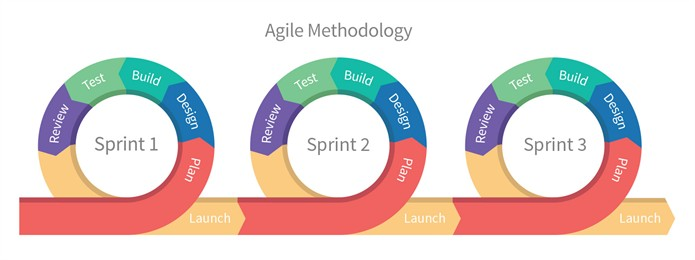
\includegraphics[trim={0 0 0 0},clip,width=1\textwidth]{Files/agile.jpg}
	\caption{Visualization of the iterations\cite{agile:figure}.}
	\label{fig: MVC}
\end{figure}

\section{Ruby on Rails} 
\vspace{-5mm}
Ruby on Rails, or simply Rails, is a server-side web application framework written in Ruby under the MIT License. Rails is a model–view–controller (MVC) framework, providing default structures for a database, a web service, and web pages. \cite{wiki:RoR}

\begin{figure}[H]
	\centering
    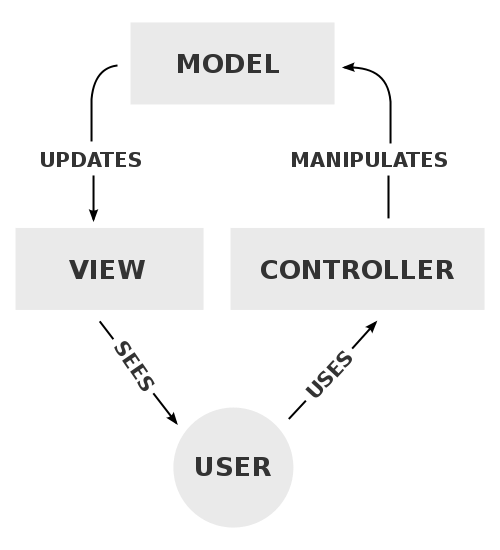
\includegraphics[trim={0 0 0 0},clip,width=0.5\textwidth]{Files/MVC.png}
    \caption{Diagram of interactions within the MVC pattern.\cite{wiki:mvc} }
    \label{fig: MVC}
\end{figure}


\textbf{The Model:}
\vspace{-5mm}
\begin{itemize}
 \setlength{\itemsep}{-5pt}
\item Contains data for the application (often linked to a database)
\item Contains state of the application (e.g. what orders a customer has)
\item  Contains all business logic
\item Notifies the View of state changes (** not true of ROR, see below)
\item No knowledge of user interfaces, so it can be reused
\end{itemize}

\textbf{The View:}
\vspace{-5mm}
\begin{itemize}
 \setlength{\itemsep}{-5pt}
\item Generates the user interface which presents data to the user
\item Passive, i.e. doesn’t do any processing
\item Views work is done once the data is displayed to the user.
\item Many views can access the same model for different reasons
\end{itemize}

\textbf{The Controller:}
\vspace{-5mm}
\begin{itemize}
 \setlength{\itemsep}{-5pt}
\item Receive events from the outside world (usually through views)
\item Interact with the model
\item Displays the appropriate view to the user
\end{itemize}

https://stackoverflow.com/questions/1931335/what-is-mvc-in-ruby-on-rails




